\scanpage{5}
\mspage{4}

\uline{Th} $f:X\to S$ morphisme \inserted{\uline{plat}} de type fini, avec $S$ loc noeth, $Y$ \deleted{un sous-\unsure{préschém.} fermé de $X$}\inserted{$\to X$ un \unsure{mor.} de type fini}.

Pour que $\prod_{X/S}Y/X$ soit représentable, il f. et s. qu'il commute aux limites projectives adiques d'anneaux artiniens\inserted{, Si $Y\to X$ \unsure{une imm.} (\uuline{imm.f.})}, et alors il est représentable par un sous-préschém. (\uuline{fermé}) de $S$.

\margin{il suffit que $Y\to X$ soit un \uuline{\unsure{monomorphisme}}}

\figure{\begin{tikzpicture}\draw (0,0)--(10,0);\end{tikzpicture}}

\deleted{\unsure{fpqc}}

\uline{Dém.} Vérifions les conditions générales du th. de représentabilité pour morphismes non ramifiés séparés

1°) $F$ faisceau pour fpqc: \deleted{\unsure{EGA IV 2}} clair EGA IV 2

2°) $F$ commute aux $\varinjlim$ d'anneaux: clair EGA IV 8

\margin{$\times$ \unsure{N.B.}}

3°) C'est la condition de commutation aux $\varprojlim$ adiques d'artiniens.

4°), 5°), 6°) Dans le cas d'un monomorphisme $F\to S$ se réduit à ceci

\margin{\figure{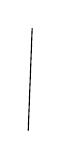
\begin{tikzpicture}\draw (0,0)--(.05,1.3);\end{tikzpicture}}}

si $A\to A'$ est un hom injectif d'artiniens \inserted{($A'/A$ fini)}

alors $F(A)\to F(A')$ est bijectif, ou même $F(A')\ne\varnothing\Rightarrow F(A)\ne\varnothing$. Il faut prouver que si $X_{A'}=Y_{A'}$, on a $X_A=Y_A$. C'est clair, car $X_A$ \deleted{\unsure{étant}} plat sur $A$, $\unsure{\underline O_{X_A}|\mathcal O_{X_A}}\deleted{\unsure{\otimes_A A}}\to\unsure{\underline O_{X_A}|\mathcal O_{X_A}}\otimes_A A'$ est injectif.

\margin{$\times$ \uline{plat}}

7°) Si $T$ sur $S$ est \deleted{\unsure{loc.}} loc. noeth., muni d'un idéal de carré nul $J$, $T_0=V(J)$, $U$ ouvert de $T$ tel que $T$ en soit l'adhérence schématique, \uline{alors} pour \deleted{$\unsure{F\subset F}$}
\diagram{\begin{tikzcd}
F(T) \arrow[r,dash] \arrow[d] & F(T_0) \arrow[d] \\
F(U) \arrow[r] & F(U_0)
\end{tikzcd}}
est cartésien.

\margin{$\times$ \uline{plat} \deleted{\uline{\unsure{Difficulté|fidèle}}}}
